\newpage
\section{Aufbau}
\label{sec:Aufbau}
Der hier untersuchte Si-Streifendetektor (EASy) der Firma Alibava besteht aus drei Komponenten.
Eine Kontroll- und eine Detektoreinheit, sowie ein Computer mit Steuer-Software.

\subsection{Detektoreinheit}
\label{sec:Detektoreinheit}
 Als Detektoreinheit wird der Si-Streifenhalbleiter und die Ausleseelektronik
 zusammengefasst. Dabei besteht der \SI{300}{\micro\meter} dicke Si-Detektor
 aus 128 einzelnen p-dotierten Streifen in dem n-dotierten Silizium.  Dieser
 Aufbau ist in Abbildung \ref{fig:schema} zu erkennen.
 \begin{figure}[htb]
   \centering
   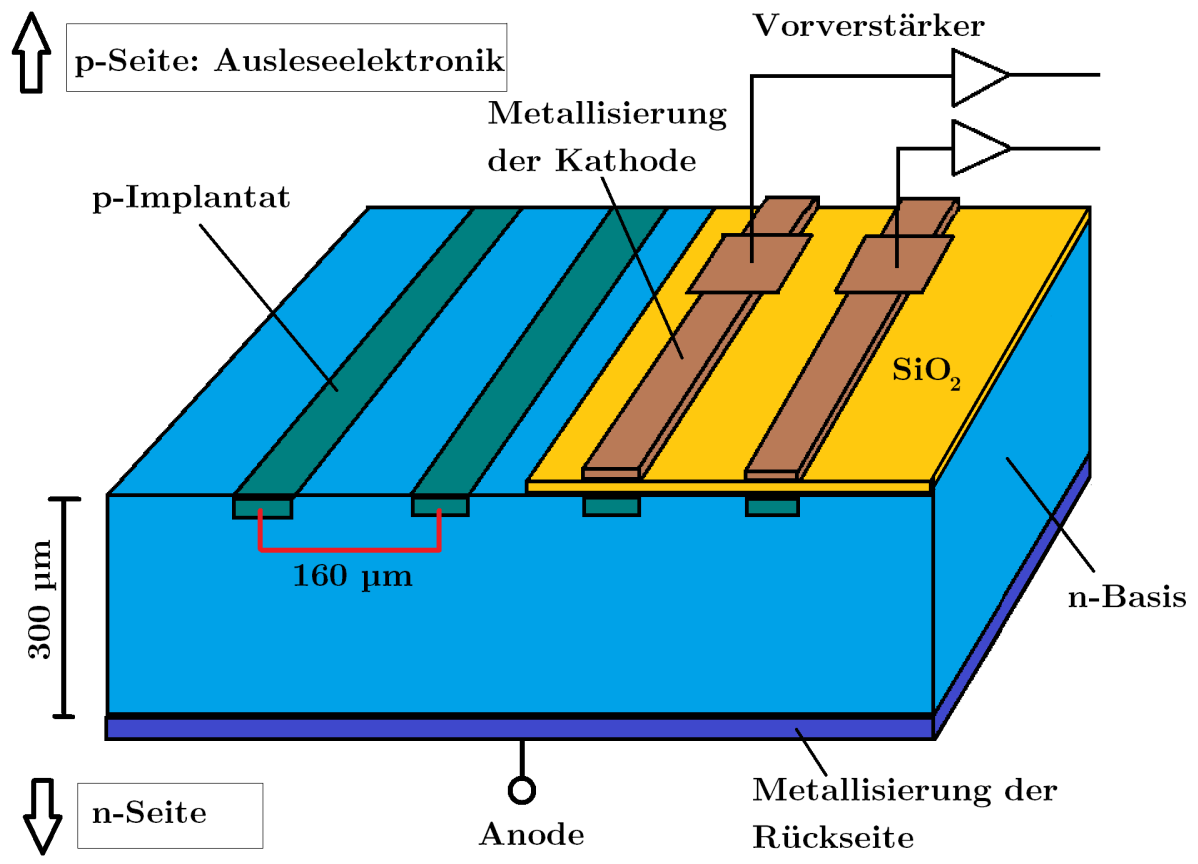
\includegraphics[width=0.7\textwidth]{images/Schema.png}
   \caption{Schematische Darstellung eines Si-Streifensensors mit Spannungsanschluss \cite{anleitung}.}
   \label{fig:schema}
 \end{figure}
Eine Schicht aus Siliziumoxid sorgt dafür, dass kein Signal aus den p-Implantaten
auf den Auslesechip überschlägt. Jeder p-Streifen ist durch Wirebonding mit der
Ausleseelektronik verbunden. Zudem bezitzen die p-Streifen durch einen Ohmschen
Wiederstand eine Verbindung zu dem Bias Ring, welcher eine Spannung an den Streifen
anlegt.
Um den Bias Ring ist ein Guard Ring zur Vermeidung von Oberflächenströmen angebracht.
In Abbildung \ref{fig:streifendetektor} ist dies an
einer makroskopischen Aufnahme deutlich gemacht.
\begin{figure}[htb]
  \centering
  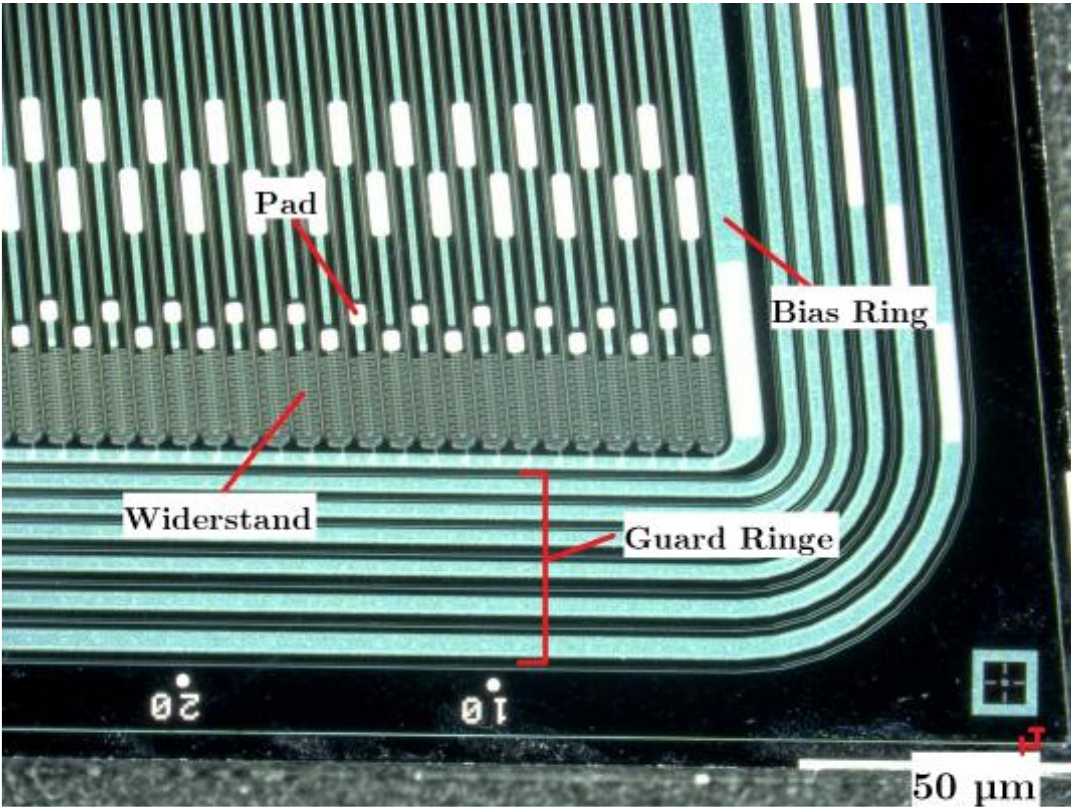
\includegraphics[width=0.5\textwidth]{images/Sensor.png}
  \caption{Makroskopische Aufnahmne eines Streifen-Detektors mit entsprechender Kennzeichnung der einzelnen Komponenten \cite{anleitung}.}
  \label{fig:streifendetektor}
\end{figure}
Die Informationen aus den einzelnen Streifen nach Durchgang eines geladenen
Teilchens werden durch einen Auslesechip zuerst verstärkt und danach in
Spannungssignale umgewandelt. Dann werden die Signale in eine Pipeline geschickt,
wo sie auf ein Triggersignal warten. Kommt dieses Triggersignal nicht, so werden
die Daten verworfen.

Dieser Aufbau funktioniert wie in Kapitel \ref{sec:Theorie} beschrieben
erst richtig, wenn der Halbleiterdetektor vollständig depletiert ist. Bei dem
EASy liegt dazu $U_\text{Dep}$ bei ungefähr \SIrange{60}{80}{\volt}. Um zu
ermitteln, inwiefern der Detektor depletiert ist, wird die Effizienz der
Ladunssammlung (CCE) bestimmt. Maximal ist diese Effizienz, wenn eine vollkommene
Depletierung ($U \ge U_\text{Dep}$) vorhanden ist. Nun kann die CCE bestimmt werden
durch
\begin{equation}
  \text{CCE}(U) = \frac{1 - \exp\left(\frac{-d_\text{c}(U)}{a}\right)}{1 - \exp\left(\frac{-D}{a}\right)}.
  \label{eqn:CCEL}
\end{equation}
Diese Formel gilt allerdings nur für Photonen, daher wird diese Messung mit dem
eingebauten Laser durchgeführt.
Hierbei ist $d_\text{c}$ die Dicke der Depletionszone, $D$ die Sensordicke und
$a$ die Eindringtiefe des Lasers in das Silizium.

\FloatBarrier
\subsection{Lasereinheit}
\label{sec:Lasereinheit}
Aus Abbildung \ref{fig:Gehäuse}ist das äußere Gehäuse des Detektors zu entnehmen.
\begin{figure}[htb]
  \centering
  \includegraphics[width=0.9\textwidth]{images/Gehäuse.png}
  \caption{Fotographie des EASy Gehäuses mit integriertem Laser und Carbon-Plätchen,
  sowie den einzelnen Anschlüssen \cite{anleitung}.}
  \label{fig:Gehäuse}
\end{figure}
Auf dem Gehäuse sitzt ein Reiter mit einem eingebauten Laser zur Untersuchung der
Detektoreigenschaften. Dieser kann in Laser(L)- oder in Quell(Q)-Position
gestellt werden, je nachdem, welche Messung durchgeführt werden soll.

Der angebrachte Laser emittiert Licht mit einer Wellenlänge von \SI{980}{\nano\meter}
mit einem Durchmesser von \SI{20}{\micro\meter}, einer Pulslänge von
\SI{5}{\nano\second} und einer Leistung von \SI{0.6}{\milli\watt}.
An dem Laser sind zwei Miktrometerschrauben angebracht, um diesen in der Vertikalen
zu fokussieren und in der Horizontalen verschieben zu können.

\FloatBarrier
\subsection{Kontrolleinheit}
Die Kontrolleinheit, in Abbildung \ref{fig:control} zu sehen, dient zur Steuerung
des Detektors. Über den Sockel mit der Aufschrift \textit{Sensor Unit} kann durch
ein  Flachbandkabel eine Verbindung zwischen Detektoreinheit und Kontrolleinheit
hergestellt werden. Zudem können für die Messungen mit dem Laser ein Glasfaserkabel,
bzw. für die Quellmessungen ein Triggerkabel angeschlossen werden. Über den
Drehknopf \textit{Diode Bias} wird eine bestimmte Vorspannung auf den Bias Ring
und somit auf die Halbleiterstreifen gegeben. Diese ist im Kontrollfenster,
zusammen mit dem auftretenden Strom abzulesen.
Auf der Rückseite der Kontrolleinheit befindet sich unter anderem ein Anschluss
für einen Kaltgerätestecker.
\begin{figure}[htb]
  \centering
  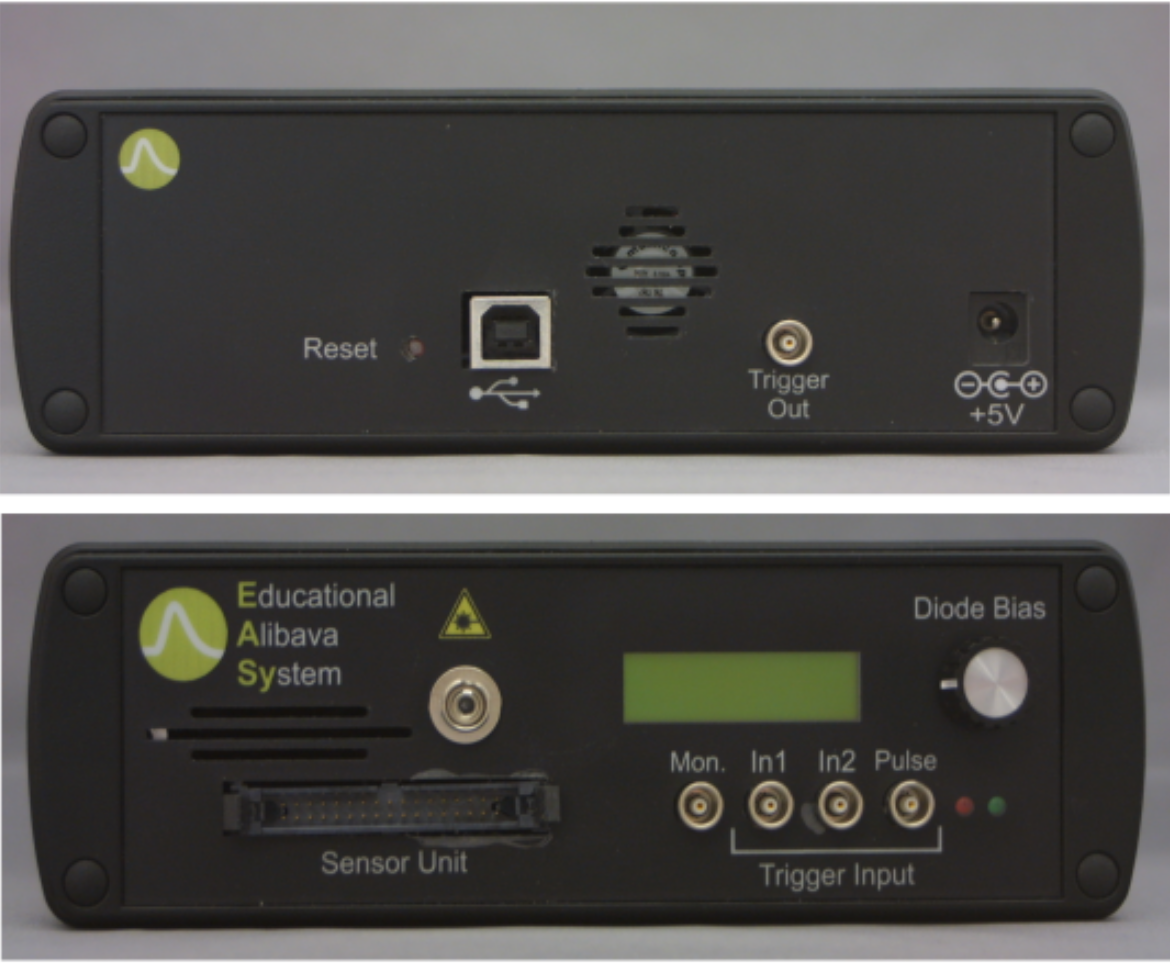
\includegraphics[width=0.4\textwidth]{images/Control.png}
  \caption{Front- und Rückansicht der Kontrolleinheit und ihrer Anschlüsse \cite{anleitung}.}
  \label{fig:control}
\end{figure}
Werden alle Bestandteile angeschlossen, so ist der Aufbau wie in Abbildung
\ref{fig:aufbau} dargestellt zu erhalten.
\begin{figure}[htb]
  \centering
  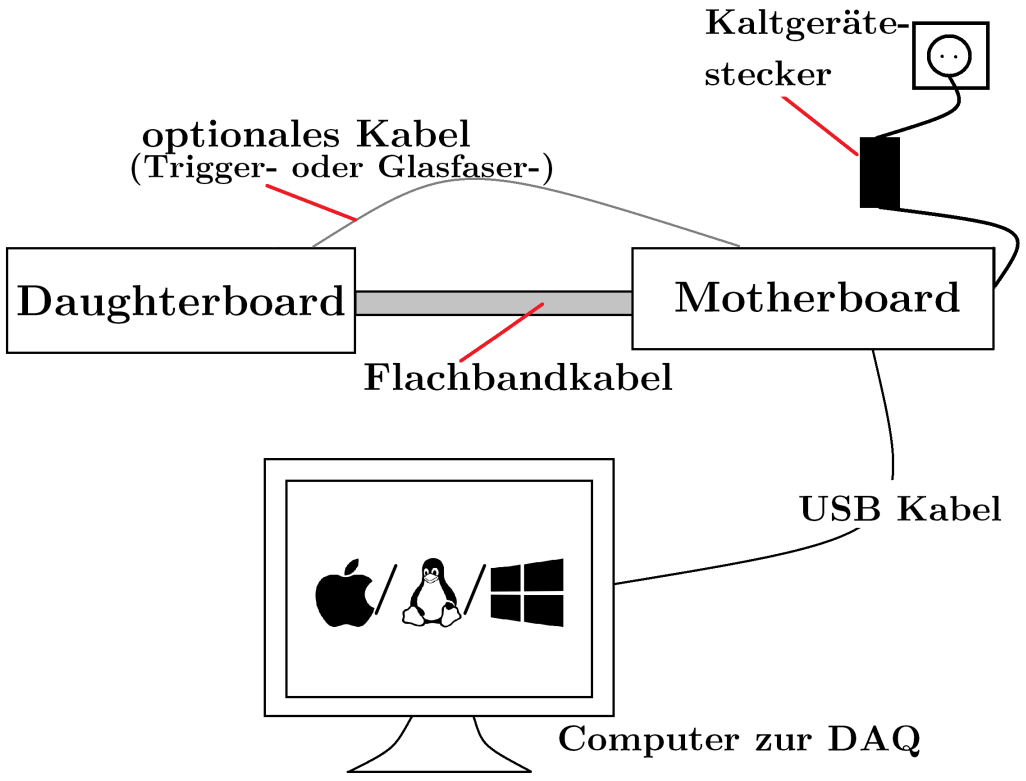
\includegraphics[width=0.5\textwidth]{images/Aufbau.png}
  \caption{Graphischer Aufbau des kompletten Versuches mit Detektoreinheit
  (Daughterbrd), Kontrolleinheit (Motherboard) und Computer \cite{anleitung}.}
  \label{fig:aufbau}
\end{figure}
Für Messungen mit der Sr-Quelle wird die Detektoreinheit zusätzlich in ein Kiste
mit Bleiabdeckung plaziert, damit keine radioaktive Strahlung nach außen gelangen
kann. Dies ist in Abbildung \ref{fig:quell} noch einmal dargestellt.
\begin{figure}[htb]
  \centering
  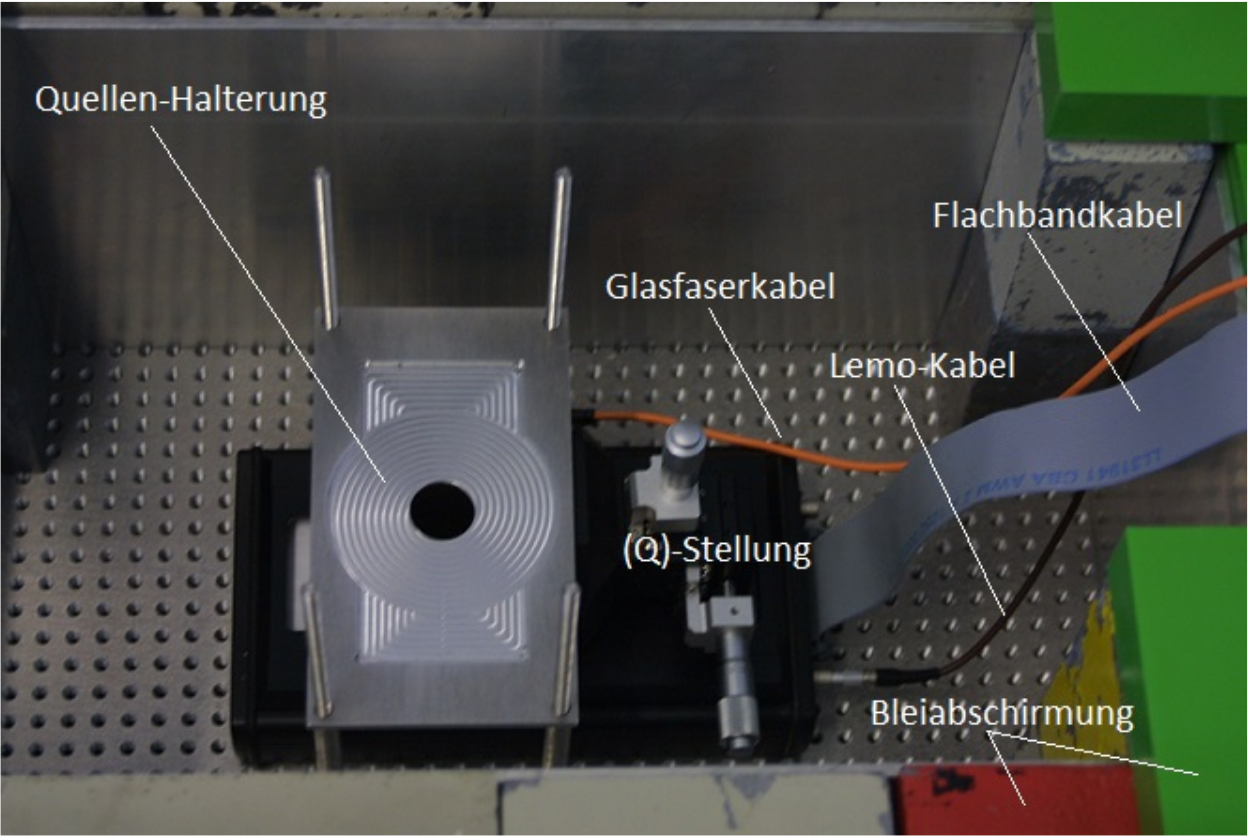
\includegraphics{images/Abschirmung.png}
  \caption{Vertikale Sicht auf die Detektoreinheit in horizontaler Bleiabschirmung \cite{anleitung}.}
  \label{fig:quell}
\end{figure}

\FloatBarrier
\section{Durchführung}
\label{sec:Durchführung}

\subsection{Messung der Strom-Spannungs-Kennlinie}
\label{sec:Kennlinie}
Zur Aufnahme einer Strom-Spannungs-Kennlinie werden die Detektor und Kontrolleinheit
an den Computer angeschlossen und das zum EASy mitgeführte Programm \textit{Alibava\_gui}
gestartet werden. Zur eigentlichen Messung muss die Vorspannung von \SI{0}{\volt} bis
einschließlich \SI{200}{\volt} in \SI{10}{\volt} Schritten durchlaufen und
der Leckstrom aufgezeichnet werden.

Dann wird eine Depletionsspannung im erhaltenen Verlauf durch Übergang von einem
sättigenden zu einer linearen Verlauf abgeschätzt. Für weitere Messungen wird
ein Wert für die Depletionsspannung gewählt, der ca. \SI{20}{\volt} größer ist als
der ermittelte Wert.

\subsection{Pedestals und Noise}
\label{sec:Auswertung_Noise}
Um Informationen über die Pedestals und Noise zu erhalten, wird eine LogData im
Ordner Pedestal und Namen Pedestal.h5 angelegt und ein \textit{Pedastal Run}
durchgeführt. Hierbei wird die Messung für 1000 Events durchgeführt.

\subsection{Kalibrationsmessung}
\label{sec:Kalibrationsmessung}
Nun wird über das Flachbandkabel ein Elektronenpuls an den Auslesechip gegeben
um die ADC-Counts in Ladung umrechnen zu können. Um eine Kalibrationskurve
aufzunehmen, wird die Option \textit{Calibration Run} gewählt und im entsprechenden
Optionsfenster die Default-Werte der Delay Einstellung wie in Abbildung
\ref{fig:calibration-durchfuehrung} zu sehen verwendet. Nun wird der Delay-Scan durchgeführt,
um eine optimale Verzögerung zwischen eingegebenem Signal und Chipauslese zu
erhalten. Anschließend ist das Maximum der entstandenen Verteilung zu suchen und
der entsprechende Wert unter \textit{Settings} und \textit{DAQ} einzutragen.
\begin{figure}[htb]
  \centering
  \includegraphics[width=0.3\textwidth]{images/Calibration.png}
  \caption{Default-Einstellungen der Messung einer Kalibrationskurve zur Bestimmung
  der besten Verzögerung zwischen gebenen Elektronenpuls und Chipauslese \cite{anleitung}.}
  \label{fig:calibration-durchfuehrung}
\end{figure}

Im zweiten Schritt werden fünf verschiedene Kanäle bzw. Streifen des Streifendetektors
ausgewählt und unter \textit{Option} im \textit{Calibration}-Menü nacheinander
eingestellt. Für jeden Streifen wird ein Run durchgeführt und die Graphik gespeichert.
Für einen der fünf Streifen wird zudem ein Run bei $U=\SI{0}{\volt}$ durchgeführt.

\FloatBarrier
\subsection{Vermessung der Streifendetektoren mittels Laser}
\label{sec:Vermessung_Laser}
Hier wird nun die Streifenstruktur des Detektors untersucht. Dies funktioniert,
da sich in der Mitte diese Streifen eine Metallisierung befindet, welche das vom
Laser emittierte Licht reflektiert und daher den Halbleiter nicht durchdringt.
Zu Beginn wird dazu die optimale Verzögerung zwischen Lasersignal und Chipauslese
bestimmt. Dafür wird unter \textit{Option} \textit{Laser Sync.} ausgewählt und
der Run durchgeführt. Aus dem Maximum der angezeigten Abhängigkeit zwischen
gemessenen ADC-Counts und Verzögerung kann nun die optimale Verzögerung abgelesen
und unter dem Formularfeld bei \textit{Laser Run} eingetragen werden.

Als nächstes wird mithilfe der horizontalen Mikrometerschraube der Peaks maximiert.
Dies ist der Fall, wenn genau ein Streifen getroffen wurde. Ab dort wird in \num{35}
\SI{10}{\micro\meter}-Schritten ein Laserscan durchgeführt und diese gespeichert.


\subsection{Bestimmung der Charge Collection Eficiency}
\label{sec:CCE}
\subsubsection{Unter Verwendung eines Lasers}
Wie im Schritt zuvor wird zu Beginn dieser Messung erst der maximale Peak mit
optimaler Verzögerung gesucht. Nun wird allerdings für je \num{1000} Events die
Spannung von \SIrange{0}{200}{\volt} in \SI{10}{\volt}-Schritten erhöht und ein
Run durchgeführt.

\subsubsection{Unter Verwendung einer Sr-Quelle}
Nach dem Umplatzierung der Detektoreinheit in einen strahlengeschützen Aufbau wird
analog zu der CCE-Bestimmung duch einen Laser die Spanung in \SI{10}{\volt}-Schritten
von \SIrange{0}{200}{\volt} erhöht. Hier werden pro Run der Datensatz auf \num{10000}
erhöht.

\subsection{Großer Quellscan}
\label{sec:Quellscan}
Für die letzte Messung wird die Spannung wie in der Messung der Strom-Spannungs-Kennlinie
auf einen Wert leicht über der Depletionsspannung gesetzt und ein \textit{RS Run} mit
einer Anzahl der Events von \num{1000000} durchgeführt und abgespeichert.

Durch ein mitgeführtes Programm werden alle \textit{.h5}-Dateien in passende .txt-Dateien
umgewandelt, damit diese für die Auswertung herangezogen werden können.
